\documentclass[a4paper, 12pt]{article}

\usepackage[top=2cm, bottom=2cm, left=2.5cm, right=2.5cm]{geometry}
\usepackage[utf8]{inputenc}
\usepackage{amsmath, amsfonts, amssymb}
\usepackage{graphicx} % inserir figuras - \includegraphics[scale=•]{•}
\usepackage{float} % ignorar regras de tipografia e inserir figura aonde queremos.
\usepackage[brazil]{babel} % Trocar Figure para Figura.
\usepackage{indentfirst}
\pagestyle{empty}


\begin{document}
\begin{figure}[H]
	
\includegraphics[scale=0.9]{UnB_CiC_Logo.jpg}
\end{figure}
\noindent\rule{\textwidth}{0.4pt}
\begin{center}
	\textbf{{\Large Introdução à Ciência da Computação - 113913}} \newline \newline
	\textbf{{\large Lista de Exercícios 3} \\
	\vspace{9pt}
	{\large Laço de Repetição For e While}} \\
	\noindent\rule{\textwidth}{0.4pt}
	\newline
\end{center}

\textbf{{\large Observações:}}
\begin{itemize}
	\item As listas de exercícios serão corrigidas por um \textbf{corretor automático}, portanto é necessário que as entradas e saídas do seu programa estejam conforme o padrão especificado em cada questão (exemplo de entrada e saída). Por exemplo, não use mensagens escritas durante o desenvolvimento do seu código como “Informe a primeira entrada”. Estas mensagens não são tratadas pelo corretor, portanto a correção irá resultar em resposta errada, mesmo que seu código esteja correto.
	\item As questões estão em \textbf{ordem de dificuldade}. Cada lista possui 7 exercícios, sendo 1 questão fácil, 3 ou 4 médias e 2 ou 3 difíceis.
	\item Assim como as listas, as provas devem ser feitas na versão Python 3 ou superior.
	\item Leia com atenção e faça \textbf{exatamente} o que está sendo pedido.
\end{itemize}
\newpage % Questão A 
\begin{center}
\textbf{{\Large Questão A - Jogo de Adivinhação}}
\end{center}
\vspace{5pt}
Um pequeno jogo de adivinhação funciona da seguinte forma: você define um número \textbf{n} e chama um amigo, que deverá adivinhar o número escolhido. Faça um programa que peça um inteiro e então fique pedindo que um usuário tente adivinhá-lo até que acerte. Em cada tentativa o programa deve dizer se o chute foi maior ou menor que o número certo.
\newline \newline
\textbf{{\large Entrada}} \newline
A primeira linha de entrada será o inteiro \textbf{\textit{n}}, que deverá ser adivinhado. As próximas linhas serão os números chutados pelo jogador, que continuará chutando números até que adivinhe o número correto.
\newline \newline
\textbf{{\large Saída}} \newline
Se o número digitado for menor que \textbf{\textit{n}} apresente a mensagem: ``O número correto é maior.''. Se o número digitado for maior que \textbf{\textit{n}} apresente a mensagem: ``O número correto é menor.''. Quando o usuário acertar o número imprima: ``Parabéns! Você acertou.''.
\newline
\begin{table}[H]
	\centering
	\begin{tabular}{|l|l|}
	\hline
	\textbf{Exemplo de Entrada} & \textbf{Exemplo de Saída} \\ \hline
	\begin{tabular}{l}
	7 \\
	5 \\
	8 \\
	7
	\end{tabular} & 
	\begin{tabular}{l}
	O número correto é maior. \\
	O número correto é menor. \\
	Parabéns! Você acertou. 
	\end{tabular} \\ \hline
	
	\begin{tabular}{l}
	5 \\
	4 \\
	5
	\end{tabular} & 
	\begin{tabular}{l}
	O número correto é maior. \\
	Parabéns! Você acertou. 
	\end{tabular} \\ \hline
	
	\begin{tabular}{l}
	-2 \\
	-1 \\
	-3 \\
	-2
	\end{tabular} & 
	\begin{tabular}{l}
	O número correto é menor. \\
	O número correto é maior. \\
	Parabéns! Você acertou. 
	\end{tabular} \\ \hline
	
	\end{tabular}
	\caption{Questão A}
	\label{tabela1}
\end{table}

\newpage % Questão B
\begin{center}
\textbf{{\Large Questão B - Sequência de Inteiros}}
\end{center}
\vspace{5pt}
Faça um programa que peça ao usuário para digitar uma sequência de inteiros. O programa deve parar quando \textbf{0} for digitado, que será desconsiderado na sequência de números lidos. No final, você deve apresentar a quantidade de números lidos, o maior inteiro e a média aritmética simples dos inteiros.
\newline \newline
\textbf{{\large Entrada}} \newline
A entrada consistirá de uma sequência de inteiros que será terminada quando o valor 0 for digitado, o qual não fará parte da sequência. É possível que a sequência não tenha nenhum número (nesse caso considere 0 como o maior número da sequência).
\newline \newline
\textbf{{\large Saída}} \newline
Apresente \textbf{\textit{x, y e z}}, um por linha, onde \textbf{\textit{x, y e z}} representam, respectivamente, a quantidade de números, o maior número e a média dos inteiros da sequência com 2 casas decimais após a vírgula.
\newline
\begin{table}[H]
	\centering
	\begin{tabular}{|l|l|}
	\hline
	\textbf{Exemplo de Entrada} & \textbf{Exemplo de Saída} \\ \hline
	\begin{tabular}{l}
	3 \\
	3 \\
	-1 \\
	-2 \\
	-4 \\
	-5 \\
	0
	\end{tabular} & 
	\begin{tabular}{l}
	6 \\
	3 \\
	-1.00
	\end{tabular} \\ \hline
	
	\begin{tabular}{l}
	-1 \\
	-2 \\
	-3 \\
	-4 \\
	-5 \\
	0
	\end{tabular} & 
	\begin{tabular}{l}
	5 \\
	-1 \\
	-3.00
	\end{tabular} \\ \hline
	
	\begin{tabular}{l}
	2 \\
	2 \\
	-2 \\
	-2 \\
	0
	\end{tabular} & 
	\begin{tabular}{l}
	4 \\
	2 \\
	0.00
	\end{tabular} \\ \hline
	\end{tabular}
	\caption{Questão B}
	\label{tabela2}
\end{table}

\newpage % Questão C
\begin{center}
\textbf{{\Large Questão C - Duplas de Inteiros}}
\end{center}
\vspace{5pt}
Faça um algoritmo para ler um valor \textbf{\textit{T}}, um valor \textbf{\textit{A}} e um valor \textbf{\textit{N}}. Leia \textbf{\textit{T}} vezes valores \textbf{\textit{A}} e \textbf{\textit{N}} e imprima a soma dos \textbf{\textit{N}} números a partir de \textbf{\textit{A}} (inclusive), para cada um dos valores \textbf{\textit{A}} e \textbf{\textit{N}} lidos. Imprima também cada um dos \textbf{\textit{N}} números a partir de \textbf{\textit{A}}, incluindo o \textbf{\textit{A}}.
\newline \newline
\textbf{{\large Entrada}} \newline
A entrada contém somente valores inteiros, sendo $\textrm{\textbf{T}} \geq \textrm{\textbf{0}}$ e $\textrm{\textbf{N}} > \textrm{\textbf{0}}$. Na primeira linha será lido o valor \textbf{\textit{T}} e nas próximas \textbf{\textit{T}} linhas serão lidos os valores de \textbf{\textit{A}} e \textbf{\textit{N}}, separados por espaço.
\newline \newline
\textbf{{\large Saída}} \newline
Escreva na tela, para cada dupla de \textbf{\textit{A}} e \textbf{\textit{N}} lidos, cada um dos \textbf{\textit{N}} números a partir de \textbf{\textit{A}}, separados por espaço. Logo em seguida imprima \textbf{\textit{X}}, onde \textbf{\textit{X}} representa a soma dos \textbf{\textit{N}} números a partir de \textbf{\textit{A}}, conforme exemplo de saída. \textbf{Não deve haver espaços em branco após o último valor de cada linha}.
\newline \newline
\textbf{{\large Nota}} \newline
Lembre-se que para ler vários valores em uma mesma linha, use \textbf{\textit{input().split()}}. Se o argumento de split for vazio, o separador das variáveis é um espaço em branco. Porém, \textbf{input lê apenas strings do teclado}, portanto você deverá converter as strings em floats. No exemplo a seguir, o usuário digita valores separados por um espaço em branco e aperta enter para enviá-los, então, o programa lê esses valores separados por espaços como strings (na ordem em que aparecem), guardados nas variáveis correspondentes e os converte para inteiros: \newline
\textbf{\textit{A, B = input().split() \newline
A, B = [int(A), int(B)] \newline
print(``\%.0f$\backslash$n\%.0f''\%(a,b))}}
\newline
\begin{table}[H]
	\centering
	\begin{tabular}{|l|l|}
	\hline
	\textbf{Exemplo de Entrada} & \textbf{Exemplo de Saída} \\ \hline
	\begin{tabular}{l}
	3 \\
	1 3 \\
	4 5 \\
	0 10 
	\end{tabular} & \begin{tabular}{l}
	1 2 3 \\
	6 \\
	4 5 6 7 8 \\
	30 \\
	0 1 2 3 4 5 6 7 8 9 \\
	45
	\end{tabular} \\ \hline
	
	\begin{tabular}{l}
	2 \\
	5 5 \\
	4 3 
	\end{tabular} & \begin{tabular}{l}
	5 6 7 8 9 \\
	35 \\
	4 5 6 \\
	15
	\end{tabular} \\ \hline
	
	\begin{tabular}{l}
	3 \\
	-1 4 \\
	-5 10 \\
	-3 1
	\end{tabular} & \begin{tabular}{l}
	-1 0 1 2 \\
	 2 \\
	-5 -4 -3 -2 -1 0 1 2 3 4 \\
	-5 \\
	-3 \\
	-3
	\end{tabular} \\ \hline
	\end{tabular}
	\caption{Questão C}
	\label{tabela3}
\end{table}

\newpage % Questão D
\begin{center}
\textbf{{\Large Questão D - Ímpares Consecutivos}}
\end{center}
\vspace{5pt}
Leia um valor inteiro \textbf{\textit{N}} que é a quantidade de casos de teste que vem a seguir. Cada caso de teste consiste de dois inteiros \textbf{\textit{X}} e \textbf{\textit{Y}}. Você deve apresentar a soma de \textbf{\textit{Y}} ímpares consecutivos a partir de \textbf{\textit{X}}, inclusive o próprio \textbf{\textit{X}} se ele for ímpar. Por exemplo: para a entrada 4 5, a saída deve ser 45, que é equivalente à: 5 + 7 + 9 + 11 + 13, para a entrada 7 4, a saída deve ser 40, que é equivalente à: 7 + 9 + 11 + 13. No final imprima também a maior e a menor soma.
\newline \newline
\textbf{{\large Entrada}} \newline 
A primeira linha de entrada é um inteiro $\textrm{\textbf{N}} > \textrm{\textbf{0}}$ que é a quantidade de casos de teste que vem a seguir. Cada caso de teste consiste em uma linha contendo dois inteiros \textbf{\textit{X}} e \textbf{\textit{Y}}, onde $\textrm{\textbf{Y}} > \textrm{\textbf{0}}$.
\newline \newline
\textbf{{\large Saída}} \newline
Imprima a soma \textbf{\textit{S}} dos \textbf{\textit{Y}} consecutivos números ímpares a partir do valor \textbf{\textit{X}}, para cada \textbf{\textit{X}} e \textbf{\textit{Y}} lidos. Imprima também a maior e a menor soma \textbf{\textit{S}}, conforme exemplo abaixo.
\newline
\begin{table}[H]
	\centering
	\begin{tabular}{|l|l|}
	\hline
	\textbf{Exemplo de Entrada} & \textbf{Exemplo de Saída} \\ \hline
	\begin{tabular}{l}
	4 \\
	-2 5 \\
	3 3 \\
	-10 3 \\
	4 4 
	\end{tabular} & \begin{tabular}{l}
	15 \\
	15 \\
	-21 \\
	32 \\
	32 \\
	-21
	\end{tabular} \\ \hline

	\begin{tabular}{l}
	3 \\
	-5 1 \\
	-3 2 \\
	-10 3 
	\end{tabular} & \begin{tabular}{l}
	-5 \\
	-4 \\
	-21 \\
	-4 \\
	-21
	\end{tabular} \\ \hline
	
	\begin{tabular}{l}
	2 \\
	-5 2 \\
	-5 4
	\end{tabular} & \begin{tabular}{l}
	-8 \\
	-8 \\
	-8 \\
	-8
	\end{tabular} \\ \hline	
	\end{tabular}
	\caption{Questão D}
	\label{tabela4}
\end{table}

\newpage % Questão E
\begin{center}
\textbf{{\Large Questão E - Fatorial e Fibonacci}}
\end{center}
\vspace{5pt}
No ocidente, a sequência de Fibonacci apareceu pela primeira vez no livro \textit{Liber Abaci} (1202) de Leonardo Fibonacci embora ela já tivesse sido descrita por gregos e indianos. Fibonacci considerou o crescimento de uma população idealizada (não realista biologicamente) de coelhos. Os números descrevem o número de casais na população de coelhos depois de \textbf{\textit{n}} meses se for suposto que:
\begin{itemize}
	\item No primeiro mês nasce apenas um casal,
	\item casais amadurecem sexualmente (e reproduzem-se) apenas após o segundo mês de vida,
	\item não há problemas genéticos no cruzamento consaguíneo,
	\item todos os meses, cada casal fértil dá a luz a um novo casal, e
	\item os coelhos nunca morrem.
\end{itemize}
\begin{figure}[H]
	\centering
	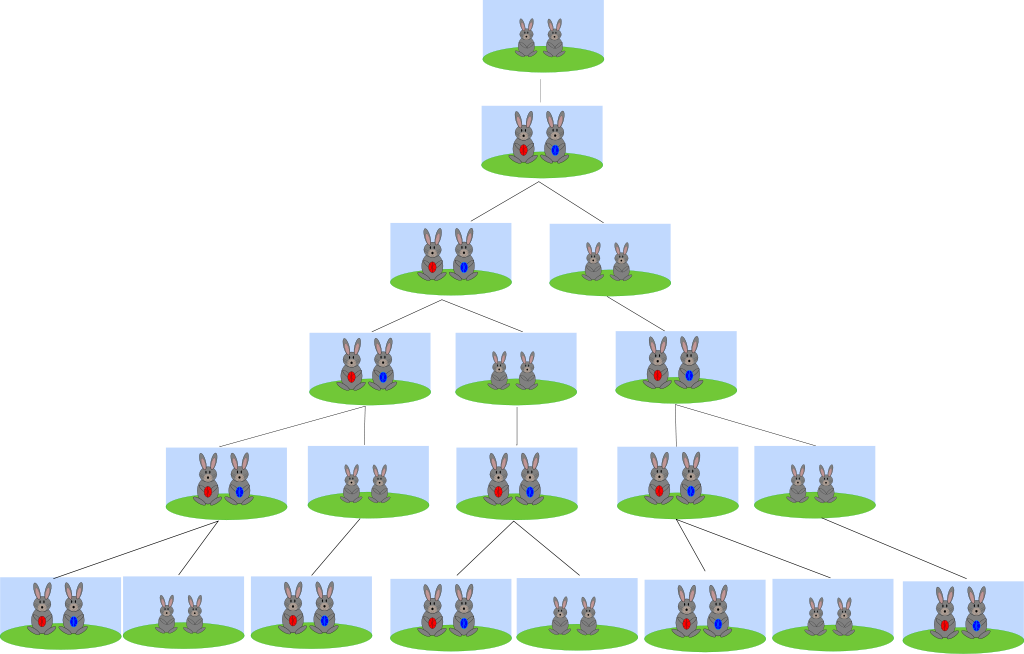
\includegraphics[scale=0.5]{Fibonacci.png}
	\caption{\textbf{\textit{Ilustração representativa da série de Fibonacci, demonstrando o crescimento populacional de coelhos.}}}
\end{figure}
Sendo $F_n$ a quantidade de casais após \textbf{\textit{n}} meses, faça um programa que, dado um inteiro positivo \textbf{\textit{n}} digitado pelo usuário, calcule o n-ésimo termo da sequência de Fibonacci usando a definição dada abaixo: 
$$F_n =
		\begin{cases}
			1;\, n = 1\ \textrm{ou}\ n = 2 \\
			F_{n-1} + F_{n-2};\, n > 2 \\
		\end{cases}
$$
Imprima também o fatorial de \textbf{\textit{n}}. \newline \newline
Caso haja um número par de casais de coelhos após \textbf{\textit{n}} meses, imprima também quantos novos casais de coelhos vão nascer no próximo mês.
\newline \newline
\textbf{{\large Entrada}} \newline
Inteiro $\textrm{\textbf{n}} > \textrm{\textbf{0}}$, onde \textbf{\textit{n}} representa os meses que passaram.
\newline \newline
\textbf{{\large Saída}} \newline
Será impresso na tela o número de casais após \textbf{\textit{n}} meses e o valor de $n!$ na mesma linha. Caso o número de casais de coelhos seja par, será impresso também, na mesma linha, quantos novos casais irão nascer no próximo mês.
\newline
\begin{table}[H]
	\centering
	\begin{tabular}{|l|l|}
	\hline
	\textbf{Exemplo de Entrada} & \textbf{Exemplo de Saída} \\ \hline
	6 & 8 720 5 \\ \hline
	1 & 1 1 \\ \hline
	10 & 55 3628800 \\ \hline
	\end{tabular}
	\caption{Questão E}
	\label{tabela5}
\end{table}

\newpage % Questão F
\begin{center}
\textbf{{\Large Questão F - Figurinhas de Harry Potter}}
\end{center}
\vspace{5pt}
Raphael e Luiza são aficionados por figurinhas de Harry Potter. Nas horas vagas, eles arrumam um jeito de jogar um ``bafo'' ou algum outro jogo que envolva tais figurinhas. Ambos também têm o hábito de trocarem as figuras repetidas com seus amigos e certo dia pensaram em uma brincadeira diferente. \newline \newline Chamaram todos os amigos e propuseram o seguinte: com as figurinhas em mãos, cada um tentava fazer uma troca com o amigo que estava mais perto seguindo a seguinte regra: cada um contava quantas figurinhas tinha. Em seguida, eles tinham que dividir as figurinhas de cada um em pilhas do mesmo tamanho, no maior tamanho que fosse possível para ambos. Então, cada um escolhia uma das pilhas de figurinhas do amigo para receber. Por exemplo, se Raphael e Luiza fossem trocar as figurinhas e tivessem respectivamente 8 e 12 figuras, ambos dividiam todas as suas figuras em pilhas de 4 figuras (Raphael teria 2 pilhas e Luiza teria 3 pilhas) e ambos escolhiam uma pilha do amigo para receber. \newline \newline 
Você pode fazer um programa para ajudá-los com essa brincadeira?
\newline \newline
\textbf{{\large Entrada}} \newline
A entrada contém uma linha com 2 inteiros \textbf{\textit{n}} $(1 \leq n \leq 1000)$ e \textbf{\textit{m}} $(1 \leq m \leq 1000)$ indicando, respectivamente, a quantidade de figurinhas que Raphael e Luiza têm para trocar.
\newline \newline
\textbf{{\large Saída}} \newline
A saída será o tamanho máximo da pilha de figurinhas que poderia ser trocada entre dois jogadores.
\newline
\begin{table}[H]
	\centering
	\begin{tabular}{|l|l|}
	\hline
	\textbf{Exemplo de Entrada} & \textbf{Exemplo de Saída} \\ \hline
	8 12 & 4 \\ \hline
	9 27 & 9 \\ \hline
	259 111 & 37 \\ \hline
	\end{tabular}
	\caption{Questão F}
	\label{tabela6}
\end{table}

\newpage % Questão G
\begin{center}
\textbf{{\Large Questão G - A Hipótese Falsa}}
\end{center}
\vspace{5pt}
Raphael e Renata estão cursando Teoria dos Números juntos, no departamento de matemática da Universidade de Brasília. Certo dia eles se deparam com a seguinte hipótese: ``Para todo inteiro positivo \textbf{\textit{n}} e \textbf{\textit{m}} temos que $n\cdot m + 1$ é um número primo''. Porém, eles percebem que essa hipótese é falsa, pois a Renata rapidamente nota que basta usar $m = n - 2$, assim:
$$n\cdot m + 1 = n(n - 2) + 1 = {(n - 1)}^2 $$ que não é primo. \newline \newline
De modo que para $\textrm{\textbf{n}} > \textrm{\textbf{2}}$, \textbf{\textit{m}} pode ser \textbf{\textit{n - 2}}. Se \textbf{\textit{n = 7}}, por exemplo, então $7\cdot 5 + 1 = 36$, que não é primo. Se $n \leq 2$, podemos usar \textbf{\textit{m = n + 2}}.
Entretanto, Raphael gosta da Renata e quer impressioná-la, apresentando não apenas qualquer contra-exemplo, mas sim o menor \textbf{\textit{m}} tal que $n\cdot m + 1$ não seja primo (para \textbf{n = 7}, também poderíamos usar \textbf{m = 1}). \newline \newline
Você pode escrever um programa para ajudá-lo, dado o inteiro \textbf{\textit{n}}?
\newline \newline
\textbf{{\large Entrada}} \newline
A entrada consistirá apenas de um inteiro \textbf{\textit{n}} $(1 \leq n \leq 1000)$ – o \textbf{\textit{n}} da hipótese.
\newline \newline
\textbf{{\large Saída}} \newline
Imprima na tela o menor $\textrm{\textbf{\textit{m}}} \geq \textrm{\textbf{\textit{1}}}$ tal que 
$\textrm{\textbf{\textit{n}}}\cdot \textrm{\textbf{\textit{m}}} + \textrm{\textbf{\textit{1}}}$ não seja um número primo. É garantido que esse \textbf{\textit{m}} existe.
\newline \newline
\textbf{{\large Nota}} \newline
Para o primeiro exemplo, $3\cdot 1 + 1 = 4$, a saída será 1. \newline
Para o segundo exemplo, $4\cdot 1 + 1 = 5$, nós não podemos imprimir 1 porque 5 é primo. Porém, m = 2 está tudo bem, visto que $4\cdot 2 + 1 = 9$, que não é primo. \newline
Para o terceiro exemplo, $10\cdot 2 + 1 = 21$, imprimimos 2.
\newline
\begin{table}[H]
	\centering
	\begin{tabular}{|l|l|}
	\hline
	\textbf{Exemplo de Entrada} & \textbf{Exemplo de Saída} \\ \hline
	3 & 1 \\ \hline
	4 & 2 \\ \hline
	10 & 2 \\ \hline
	\end{tabular}
	\caption{Questão G}
	\label{tabela7}
\end{table}
\end{document}